% vim: set tw=78 sts=2 sw=2 ts=8 aw et ai:

Wireless Sensor Networks(WSNs) consist of numerous autonomous sensors that are
capable of monitoring the environment in which they are placed using various
sensors. Such a network would be usefull for monitoring different things such
as polution levels
in a city or assess poisonous gases, or might be able to sense vibrations in order 
to predict an earthquake. 

A wireless sensor network will contain many nodes, anywhere from a couple of
hundred sensors to several thousands of nodes. Each of these nodes has one or
more sensors incorporated for collecting information about the environment, the number of
sensors is limited
by the size and power consumption. Sensors also have a microcontroller 
to process the data from the sensor and a transceiver to be able send to some 
sink-node the data it collected. They are usually powered by some sort of battery 
although solar cells and capacitors have also been used.

Each sensor device collects data from its location and sends it to the base station,
from where data from the whole network can be collected. A usual WSN is
presented in \figref{img:wsn}. It is very power
consuming to send data over long distances as the transceiver will need to
amplify the power more so this should be avoided if possible by sending data to
closer nodes. From this need of preserving the power 
arised a need of routing protocols for these
networks: instead of sending data directly to the base station, the nodes
group in an hierarchical way so that each node will send data to a cluster
head that is very close, which then sends it to the base station or to a higher
order cluster head.

\fig{img/WSN.pdf}{img:wsn}{WSN}
%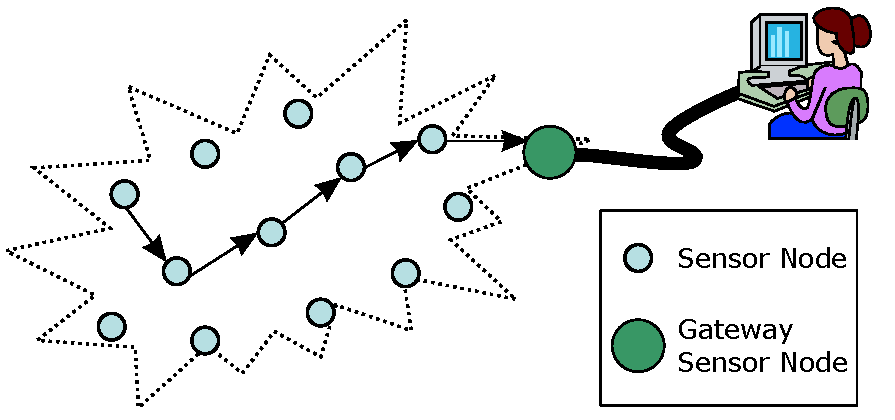
\includegraphics{img/WSN.pdf}

In this paper we will present some of the existing wireless network
simulators emphasizing what we believe to be their strenghts and weaknesses. 
In section 2.1 we discuss about NS-2 simulator, in section J-sim we present
J-sim and then we take a look at TOSSIM simulator. Based on these observations
we introduce in section 4, the WSN simulator we will implement which
encompasses most of these simulators' strenghts and adds some new features
for wireless network simulators.
